\documentclass[a4paper, 11pt]{article}
\usepackage{comment} % enables the use of multi-line comments (\ifx \fi) 
\usepackage{fullpage} % changes the margin
\usepackage{listings}
\usepackage{framed}
\usepackage{graphicx}
\graphicspath{{/}}

\lstdefinestyle{mystyle}{
	basicstyle=\small,
	breaklines,
	frame=single
}

\lstset{style=mystyle}
\begin{document}
%Header-Make sure you update this information!!!!
\noindent
\large\textbf{Homework 3} \hfill \textbf{Anirudh Ganesh} \\
\normalsize CSE 5523  \\
Prof. Mikhail Belkin \\
TA: Siyuan Ma \hfill Due Date: 04/17/18

\section*{Problem 1}

\textbf{Question :} Implement gradient descent (Richardson iteration) for the kernel learning problem 2 in previous homework. Observe how the test error changes depending upon the number of iterations on train.


\textbf{Code :}

\begin{lstlisting}[language=Python]
def iterative(n):
    K1=np.zeros([2000,2000],dtype=float)
    for i in range(0,2000):
        for j in range(0,2000):
            K1[i,j]=GaussianKernel(data_scaled_shuffle[i,:],data_scaled_shuffle[j,:],final_sigma2)


    learning_rate = 1e-3
    alphast = np.zeros(2000)
    alphast1 = np.zeros(2000)

    for i in range(n):
        alphast = alphast1
        alphast1 = alphast - learning_rate*(np.matmul(K1,alphast) - output_shuffle)

    alphas = alphast1

    cnt2=0
    tscore=0             
    for i in range(0,2000):
      sum1=0
      for j in range(0,2000):
          sum1=sum1+alphas[j]*GaussianKernel(data_scaled_shuffle[j,:],data_test_scaled[i,:],final_sigma2)
      if(sum1<0):
          predict=-1
      else:
          predict=1
      if(predict==y[i]):
          cnt2=cnt2+1
    return cnt2/2000

\end{lstlisting}

\textbf{Output :}
\begin{verbatim}
2 iterations, Test Score: 0.9125
5 iterations, Test Score: 0.9265
10 iterations, Test Score: 0.927
20 iterations, Test Score: 0.927
\end{verbatim}

\textbf{Observation :} For the given problem, the problem seems to converge to 0.927 in around 5-10 iterations and stabilizes there.

\clearpage

\section*{Problem 2}
\textbf{Question :} Apply (1) decision trees, (2) bagged, (3) boosted decision trees to the digits dataset from Homework 2. (You may use standard libraries.) Use appropriate cross-validation on the training set. Compare performance.

\subsection*{Decision Trees}
\textbf{Code :}
\begin{lstlisting}[language=Python]
mat = sio.loadmat('79.mat')
arr = mat['d79']
arr.reshape(2000,28,28)

y = np.zeros(2000)
for i in range (0,2000):
    if(i<1000):
        y[i] = 7
    else:
        y[i] = 9
        
mat1 = sio.loadmat('test79.mat')
data_test = mat1['d79']
data_test.reshape(2000,28,28)
clf = tree.DecisionTreeClassifier()
clf.fit(arr,y)

cnt = 0
for i in range(0,2000):
    if(i<1000):
        if(clf.predict(data_test[i].reshape(1, -1))[0] == 7.0):
            cnt+=1
    else:
        if(clf.predict(data_test[i].reshape(1, -1))[0] == 9.0):
            cnt+=1

print(`Test Score: {}'.format(cnt/2000))

\end{lstlisting}

\textbf{Output :}
\begin{verbatim}
Test Score: 0.943
\end{verbatim}

\subsection*{Bagging}
\textbf{Code :}
\begin{lstlisting}[language=Python]
mat = sio.loadmat('79.mat')
arr = mat['d79']
arr.reshape(2000,28,28)

y = np.zeros(2000)
for i in range (0,2000):
    if(i<1000):
        y[i] = 7
    else:
        y[i] = 9
        
mat1 = sio.loadmat('test79.mat')
data_test = mat1['d79']
data_test.reshape(2000,28,28)
clf2 = BaggingClassifier()
clf2.fit(arr,y)

cnt = 0
for i in range(0,2000):
    if(i<1000):
        if(clf2.predict(data_test[i].reshape(1, -1))[0] == 7.0):
            cnt+=1
    else:
        if(clf2.predict(data_test[i].reshape(1, -1))[0] == 9.0):
            cnt+=1

print(`Test Score: {}'.format(cnt/2000))

\end{lstlisting}

\textbf{Output :}
\begin{verbatim}
Test Score: 0.956
\end{verbatim}

\subsection*{Boosting}

\textbf{Code :}
\begin{lstlisting}[language=Python]
mat = sio.loadmat('79.mat')
arr = mat['d79']
arr.reshape(2000,28,28)

y = np.zeros(2000)
for i in range (0,2000):
    if(i<1000):
        y[i] = 7
    else:
        y[i] = 9
        
mat1 = sio.loadmat('test79.mat')
data_test = mat1['d79']
data_test.reshape(2000,28,28)
clf3 = AdaBoostClassifier(clf)
clf3.fit(arr,y)

cnt = 0
for i in range(0,2000):
    if(i<1000):
        if(clf3.predict(data_test[i].reshape(1, -1))[0] == 7.0):
            cnt+=1
    else:
        if(clf3.predict(data_test[i].reshape(1, -1))[0] == 9.0):
            cnt+=1

print(`Test Score: {}'.format(cnt/2000))

\end{lstlisting}

\textbf{Output :}
\begin{verbatim}
Test Score: 0.9625
\end{verbatim}

\section*{Problem 3}

\textbf{Question :} 1. Implement PCA and apply it to the digit data, reducing the dimension to two. Visualize the data after dimensionality reduction using colors for different classes.
2. Produce pictures of ``eigendigits'' for the dataset combining both classes and for each class separately. Observations?

\textbf{Code :}

\begin{lstlisting}[language=python]

mat = sio.loadmat('79.mat')
arr = mat['d79']
arr.reshape(2000,784)

y = np.zeros(2000)
for i in range (0,2000):
    if(i<1000):
        y[i] = 7
    else:
        y[i] = 9

cov_mat = np.cov(arr.T)
eig_vals, eig_vecs = np.linalg.eig(cov_mat)
u,s,v = np.linalg.svd(X_std.T)
for ev in eig_vecs:
    np.testing.assert_array_almost_equal(1.0, np.linalg.norm(ev))

eig_pairs = [(np.abs(eig_vals[i]), eig_vecs[:,i]) for i in range(len(eig_vals))]

eig_pairs.sort()
eig_pairs.reverse()

Y = X_std.dot(matrix_w)
traces = []

for name in [7,9]:

    trace = Scatter(
        x=Y[y==name,0],
        y=Y[y==name,1],
        mode='markers',
        name=name,
        marker=Marker(
            size=12,
            line=Line(
                color='rgba(217, 217, 217, 0.14)',
                width=0.5),
            opacity=0.8))
    traces.append(trace)


data = Data(traces)

fig = Figure(data=data)
plt.plot(fig)


\end{lstlisting}


\textbf{Output :}\\
\begin{figure}[h]
\centering
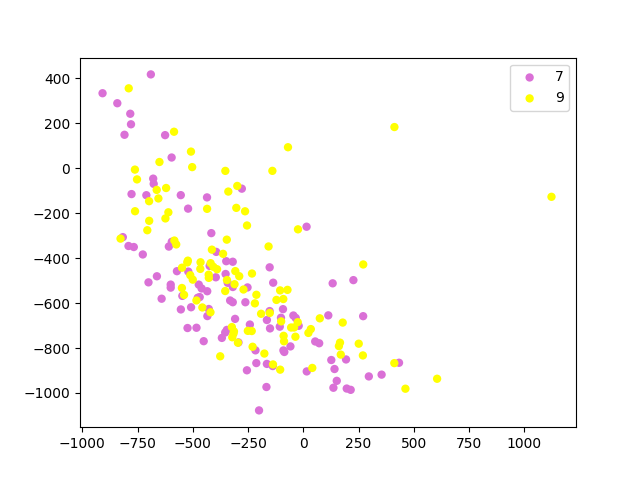
\includegraphics[width=\linewidth]{PCA}
\end{figure}
\subsection*{Eigendigits}
\begin{lstlisting}[language=python]
x = eig_vecs[:,0]*255.0
x.reshape(28,28)
x = np.array(x, dtype='uint8').reshape(28,28)
print(x.shape)
plt.imshow(x, cmap='gray')
plt.show()

x = eig_vecs[:,1]*255.0
x.reshape(28,28)
x = np.array(x, dtype='uint8').reshape(28,28)
print(x.shape)
plt.imshow(x, cmap='gray')
plt.show()
\end{lstlisting}
\clearpage
\textbf{Output :}\\
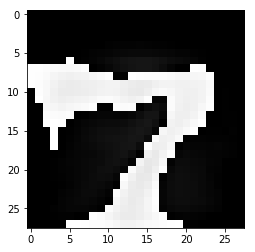
\includegraphics[scale=0.8]{eigendigit7}
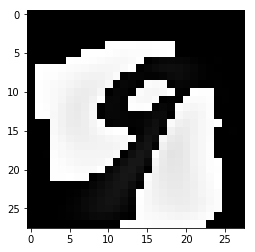
\includegraphics[scale=0.8]{eigendigit9}

\clearpage

\section*{Problem 4}

\textbf{Question :} Apply k-means clustering to the digits dataset for k= 2, 5, 10, 50. How well does it identify the different digits?


\textbf{Code :}
\begin{lstlisting}[language=Python]

def kmeams(n):
    kmeans = KMeans(n_clusters=n, random_state=0).fit(mat)
    labs=kmeans.labels_
    arr1 = np.zeros((n,2))
    arr2 = np.zeros(n)
    for i in range (0,2000):
        if(i<1000):
            arr1[labs[i]][0]=arr1[labs[i]][0]+1
        else:
            arr1[labs[i]][1]=arr1[labs[i]][1]+1
    for i in range (0,n):
        if(arr1[i][0]>arr1[i][1]):
            arr2[i]=7
        else:
            arr2[i]=9
    predictions = kmeans.predict(t.reshape(2000,-1).astype(float))
    cnt=0
    for i in range (0,2000):
        if(i<1000):
            if(arr2[predictions[i]]==7):
                cnt+=1
        else:
            if(arr2[predictions[i]]==9):
                cnt+=1
    print(cnt/2000)
\end{lstlisting}

\textbf{Output :}
\begin{verbatim}
2 clusters, Test Score: 0.5945
5 clusters, Test Score: 0.7280
10 clusters, Test Score: 0.8090
50 clusters, Test Score: 0.9265
\end{verbatim}


\end{document}
